\section{Architecture}
%
This section introduces the architecture of the currently distributed version of PostgreSQL \remark{current version of PostgreSQL}.
%
Furthermore it is shown how the architecture looks after the refactoring and implementation of the new algorithm.
%
\subsection{Current architecture}

\remark{This is one HUGE paragraph. Split it :-)}

%
In the current version of PostgreSQL the access control module is not identifiable as a stand-alone module in the backend code of the DBMS.
%
\remark{Figure~\ref{figure:postgresql:architecture}} shows a flowchart of the backend of PostgreSQL. The flowchart shows backend's behaviour.
%
There are two types of queries: \emph{utility queries} and \emph{non-utility queries}.
%
Utility queries include all queries that modify the structure of the database, e.g., adding a new table or view, creating a new trigger, or modifying the access control policy.
%
Non-utility queries on the other hand, modify the data in the underlying database structure, such as, add tuples, update tuples, or delete tuples.
%
The main difference between the former and the latter is that utility commands \remark{commands?queries?} are, in general, \emph{non-optimizable}. \remark{Undefined? True? -> Defined and true in the backend :) Should I add the comments from the backend here? }
%
\remark{The thesis must be self-contained. All the specific terminology must be explained and defined before use.}
%
That means it makes no sense to rewrite and optimize them, since there is generally no room for optimization.

Non-utility commands however go through \remark{are processed in?} several stages of \remark{in?} the backend, where they are rewritten, plans are generated, the optimal plan is chosen and finally it is executed.
%
Further the access control mechanism consists of different functions and code areas \remark{?} within functions, which are distributed among the modules.
%
Access control decisions can be made in any of the the following: Traffic cop, Executor, or in the module that handles the utility queries. \remark{undefined}
%
The functions making these decisions, however also prepare the system for the upcoming change, by, e.g., returning address where a new table is allocated, or returning the id of a already created trigger. \remark{?}
%
Due to the distribution and inconsistency \remark{?} of the access control mechanism, there is no uniform interface that can be called for such a decision.
%
Furthermore  the mechanism is, at some points, deeply connected with the internals of the database, making the implementation of a new mechanism nearly impossible without refactoring the code.
%
\begin{figure}[!ht]
  \centering
    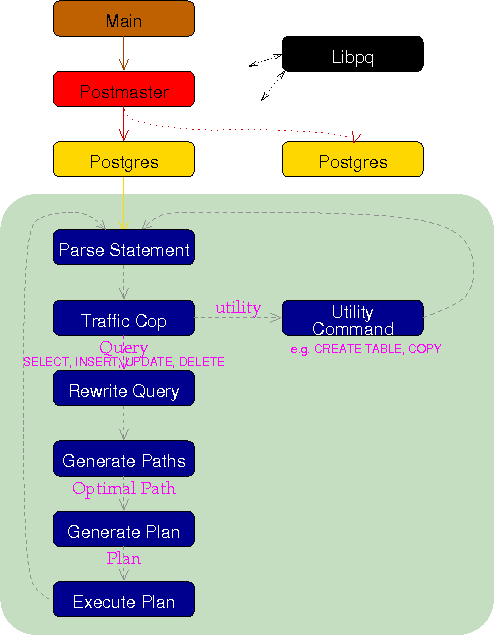
\includegraphics[width=1\textwidth]{img/backend_flowchart.png}
    \caption{Backend Flowchart PostgreSQL \protect \footnotemark}\label{figure:postgresql:architecture}
\end{figure}
%
\footnotetext{\url{http://www.postgresql.org/developer/backend}}
%
\FloatBarrier
%
\subsection{Refactoring}
%
After analyzing the backend, by executing each type of query and following the backend throught the process with a debugger, all the functions or code regions relevant to making access control decisions was identified.
%
This identification allowed to gradually move the code to an external module and build a uniform interface which is called inside the traffic cop, when the backend expects a decision. 
%
The building of a uniform interface however introduced several engineering challenges.
%
The first decision was to create a stand-alone module in the backend of PostgreSQL, which allows developers to clearly identify the code that is responsible for authorizing any type of query.
%
Second we built an interface, that can be called from any module, when requiring an access control decision.
%
Any function that calls this interface will pass all the data needed to make the decision.
%
Depending on the data received the interface internally calls the functions that were previously distributed among the modules.
%
This allows for future developers to gradually implement a new algorithm, by identifying the query received, and either return the result of a new algorithm, or call the original function responsible for the query.
%
Further we added a stack that at any point of the execution of the database system, holds all queries that are not yet completed.
%
This allows developers to always have a clear view on the state of the database system.
%
After the process of refactoring it is possible to integrate any access control mechanism as a plug-in.